\documentclass[10pt,letterpaper]{article}
\usepackage[margin=.62in]{geometry}
\usepackage{fontspec,xeCJK,amsmath,amssymb,array,booktabs,xcolor,tikz,hyperref}
\setmainfont{Helvetica Neue}
\setCJKmainfont{PingFang SC}
\usetikzlibrary{arrows.meta,positioning}
\definecolor{ink}{HTML}{172B37}
\definecolor{muted}{HTML}{425860}
\definecolor{teal}{HTML}{006D70}
\definecolor{tint}{HTML}{E4F2EF}
\definecolor{amber}{HTML}{955523}
\definecolor{sand}{HTML}{F6EADF}
\definecolor{paper}{HTML}{F3F6F6}
\hypersetup{colorlinks=true,urlcolor=teal,pdftitle={LLC Prefetching: V1 vs. Newest}}
\setlength{\parindent}{0pt}
\setlength{\parskip}{5pt}
\pagestyle{plain}
\color{ink}

% Generated by make_v1_newest_figures.py from per_region.csv and pooled.csv.
\newcommand{\ComparisonRows}{0/90M V1/amber,1/90M Newest/teal,2/110M V1/amber,3/110M Newest/teal,4/410M V1/amber,5/410M Newest/teal,6/430M V1/amber,7/430M Newest/teal,8/450M V1/amber,9/450M Newest/teal,10/Pooled V1/amber,11/Pooled Newest/teal}
\newcommand{\CapQuality}{0/0/{2,000}/sand,1/0/{495}/sand,2/0/{489}/sand,3/0/{24.75}/sand,4/0/{98.79}/sand,5/0/{0.754}/sand,6/0/{0.744}/sand,0/1/{2,000}/tint,1/1/{1,619}/tint,2/1/{876}/tint,3/1/{80.95}/tint,4/1/{54.11}/tint,5/1/{2.465}/tint,6/1/{1.334}/tint,0/2/{2,000}/sand,1/2/{433}/sand,2/2/{385}/sand,3/2/{21.65}/sand,4/2/{88.91}/sand,5/2/{0.666}/sand,6/2/{0.592}/sand,0/3/{2,000}/tint,1/3/{1,833}/tint,2/3/{863}/tint,3/3/{91.65}/tint,4/3/{47.08}/tint,5/3/{2.820}/tint,6/3/{1.328}/tint,0/4/{1,571}/sand,1/4/{214}/sand,2/4/{196}/sand,3/4/{13.62}/sand,4/4/{91.59}/sand,5/4/{1.579}/sand,6/4/{1.446}/sand,0/5/{2,000}/tint,1/5/{1,714}/tint,2/5/{965}/tint,3/5/{86.30}/tint,4/5/{55.91}/tint,5/5/{12.649}/tint,6/5/{7.122}/tint,0/6/{2,000}/sand,1/6/{808}/sand,2/6/{765}/sand,3/6/{40.40}/sand,4/6/{94.68}/sand,5/6/{0.343}/sand,6/6/{0.325}/sand,0/7/{2,000}/tint,1/7/{748}/tint,2/7/{615}/tint,3/7/{37.40}/tint,4/7/{82.22}/tint,5/7/{0.317}/tint,6/7/{0.261}/tint,0/8/{2,000}/sand,1/8/{645}/sand,2/8/{600}/sand,3/8/{32.25}/sand,4/8/{93.02}/sand,5/8/{1.415}/sand,6/8/{1.316}/sand,0/9/{2,000}/tint,1/9/{1,578}/tint,2/9/{929}/tint,3/9/{79.05}/tint,4/9/{58.89}/tint,5/9/{3.461}/tint,6/9/{2.038}/tint,0/10/{9,571}/sand,1/10/{2,595}/sand,2/10/{2,435}/sand,3/10/{27.11}/sand,4/10/{93.83}/sand,5/10/{0.610}/sand,6/10/{0.572}/sand,0/11/{10,000}/tint,1/11/{7,492}/tint,2/11/{4,248}/tint,3/11/{75.07}/tint,4/11/{56.61}/tint,5/11/{1.761}/tint,6/11/{0.998}/tint}
\newcommand{\CapCache}{0/0/{28.38}/sand,1/0/{71.62}/sand,2/0/{16.197}/sand,3/0/{0.548581}/sand,4/0/{1.8229}/sand,5/0/{4.297}/sand,0/1/{28.18}/tint,1/1/{71.82}/tint,2/1/{16.254}/tint,3/1/{0.548202}/tint,4/1/{1.8241}/tint,5/1/{4.258}/tint,0/2/{38.47}/sand,1/2/{61.53}/sand,2/2/{15.939}/sand,3/2/{0.483800}/sand,4/2/{2.0670}/sand,5/2/{4.224}/sand,0/3/{38.47}/tint,1/3/{61.53}/tint,2/3/{16.005}/tint,3/3/{0.484160}/tint,4/3/{2.0654}/tint,5/3/{4.176}/tint,0/4/{60.59}/sand,1/4/{39.41}/sand,2/4/{3.338}/sand,3/4/{0.853471}/sand,4/4/{1.1717}/sand,5/4/{0.956}/sand,0/5/{62.95}/tint,1/5/{37.05}/tint,2/5/{3.146}/tint,3/5/{0.855701}/tint,4/5/{1.1686}/tint,5/5/{0.887}/tint,0/6/{0.32}/sand,1/6/{99.68}/sand,2/6/{58.712}/sand,3/6/{0.195796}/sand,4/6/{5.1074}/sand,5/6/{15.315}/sand,0/7/{0.26}/tint,1/7/{99.74}/tint,2/7/{58.750}/tint,3/7/{0.195788}/tint,4/7/{5.1076}/tint,5/7/{15.318}/tint,0/8/{45.95}/sand,1/8/{54.05}/sand,2/8/{11.293}/sand,3/8/{0.639618}/sand,4/8/{1.5634}/sand,5/8/{3.022}/sand,0/9/{46.04}/tint,1/9/{53.96}/tint,2/9/{11.242}/tint,3/9/{0.634198}/tint,4/9/{1.5768}/tint,5/9/{2.969}/tint,0/10/{22.89}/sand,1/10/{77.11}/sand,2/10/{21.096}/sand,3/10/{0.426173}/sand,4/10/{11.7323}/sand,5/10/{27.813}/sand,0/11/{23.00}/tint,1/11/{77.00}/tint,2/11/{21.080}/tint,3/11/{0.425801}/tint,4/11/{11.7426}/tint,5/11/{27.608}/tint}
\newcommand{\NativeQuality}{0/0/{2,846}/sand,1/0/{565}/sand,2/0/{559}/sand,3/0/{19.92}/sand,4/0/{98.94}/sand,5/0/{0.860}/sand,6/0/{0.851}/sand,0/1/{25,036}/tint,1/1/{20,492}/tint,2/1/{10,983}/tint,3/1/{83.13}/tint,4/1/{53.19}/tint,5/1/{31.196}/tint,6/1/{16.720}/tint,0/2/{2,761}/sand,1/2/{440}/sand,2/2/{391}/sand,3/2/{15.97}/sand,4/2/{88.89}/sand,5/2/{0.677}/sand,6/2/{0.601}/sand,0/3/{17,978}/tint,1/3/{13,407}/tint,2/3/{7,016}/tint,3/3/{75.85}/tint,4/3/{52.08}/tint,5/3/{20.625}/tint,6/3/{10.793}/tint,0/4/{1,571}/sand,1/4/{214}/sand,2/4/{196}/sand,3/4/{13.62}/sand,4/4/{91.59}/sand,5/4/{1.579}/sand,6/4/{1.446}/sand,0/5/{5,129}/tint,1/5/{3,894}/tint,2/5/{2,255}/tint,3/5/{76.19}/tint,4/5/{57.75}/tint,5/5/{28.738}/tint,6/5/{16.642}/tint,0/6/{6,064}/sand,1/6/{2,563}/sand,2/6/{2,435}/sand,3/6/{42.27}/sand,4/6/{95.01}/sand,5/6/{1.088}/sand,6/6/{1.033}/sand,0/7/{133,815}/tint,1/7/{56,555}/tint,2/7/{44,279}/tint,3/7/{42.28}/tint,4/7/{78.28}/tint,5/7/{24.003}/tint,6/7/{18.793}/tint,0/8/{4,462}/sand,1/8/{963}/sand,2/8/{889}/sand,3/8/{21.72}/sand,4/8/{92.26}/sand,5/8/{2.112}/sand,6/8/{1.950}/sand,0/9/{14,418}/tint,1/9/{11,201}/tint,2/9/{6,425}/tint,3/9/{78.20}/tint,4/9/{57.19}/tint,5/9/{24.570}/tint,6/9/{14.094}/tint,0/10/{17,704}/sand,1/10/{4,745}/sand,2/10/{4,470}/sand,3/10/{26.85}/sand,4/10/{94.19}/sand,5/10/{1.115}/sand,6/10/{1.051}/sand,0/11/{196,376}/tint,1/11/{105,549}/tint,2/11/{70,958}/tint,3/11/{54.08}/tint,4/11/{67.00}/tint,5/11/{24.809}/tint,6/11/{16.679}/tint}
\newcommand{\NativeCache}{0/0/{28.25}/sand,1/0/{71.75}/sand,2/0/{16.197}/sand,3/0/{0.548532}/sand,4/0/{1.8230}/sand,5/0/{4.350}/sand,0/1/{41.55}/tint,1/1/{58.45}/tint,2/1/{13.233}/tint,3/1/{0.576022}/tint,4/1/{1.7360}/tint,5/1/{4.381}/tint,0/2/{38.44}/sand,1/2/{61.56}/sand,2/2/{15.946}/sand,3/2/{0.483530}/sand,4/2/{2.0681}/sand,5/2/{4.275}/sand,0/3/{47.71}/tint,1/3/{52.29}/tint,2/3/{13.611}/tint,3/3/{0.505877}/tint,4/3/{1.9768}/tint,5/3/{4.226}/tint,0/4/{60.59}/sand,1/4/{39.41}/sand,2/4/{3.338}/sand,3/4/{0.853471}/sand,4/4/{1.1717}/sand,5/4/{0.956}/sand,0/5/{66.89}/tint,1/5/{33.11}/tint,2/5/{2.823}/tint,3/5/{0.863222}/tint,4/5/{1.1585}/tint,5/5/{0.947}/tint,0/6/{1.03}/sand,1/6/{98.97}/sand,2/6/{58.295}/sand,3/6/{0.196805}/sand,4/6/{5.0812}/sand,5/6/{15.458}/sand,0/7/{18.80}/tint,1/7/{81.20}/tint,2/7/{47.832}/tint,3/7/{0.215747}/tint,4/7/{4.6351}/tint,5/7/{20.180}/tint,0/8/{46.33}/sand,1/8/{53.67}/sand,2/8/{11.251}/sand,3/8/{0.639639}/sand,4/8/{1.5634}/sand,5/8/{3.168}/sand,0/9/{54.36}/tint,1/9/{45.64}/tint,2/9/{9.571}/tint,3/9/{0.663696}/tint,4/9/{1.5067}/tint,5/9/{3.069}/tint,0/10/{23.24}/sand,1/10/{76.76}/sand,2/10/{21.006}/sand,3/10/{0.427080}/sand,4/10/{11.7074}/sand,5/10/{28.208}/sand,0/11/{36.48}/tint,1/11/{63.52}/tint,2/11/{17.414}/tint,3/11/{0.454007}/tint,4/11/{11.0130}/tint,5/11/{32.802}/tint}
\newcommand{\SmallQuality}{0/0/{300}/sand,1/0/{80}/sand,2/0/{78}/sand,3/0/{26.67}/sand,4/0/{97.50}/sand,5/0/{0.122}/sand,6/0/{0.119}/sand,0/1/{300}/tint,1/1/{193}/tint,2/1/{120}/tint,3/1/{64.33}/tint,4/1/{62.18}/tint,5/1/{0.294}/tint,6/1/{0.183}/tint,0/2/{300}/sand,1/2/{41}/sand,2/2/{41}/sand,3/2/{13.67}/sand,4/2/{100.00}/sand,5/2/{0.063}/sand,6/2/{0.063}/sand,0/3/{300}/tint,1/3/{295}/tint,2/3/{120}/tint,3/3/{98.33}/tint,4/3/{40.68}/tint,5/3/{0.454}/tint,6/3/{0.185}/tint,0/4/{300}/sand,1/4/{71}/sand,2/4/{63}/sand,3/4/{23.67}/sand,4/4/{88.73}/sand,5/4/{0.524}/sand,6/4/{0.465}/sand,0/5/{300}/tint,1/5/{250}/tint,2/5/{148}/tint,3/5/{83.33}/tint,4/5/{59.20}/tint,5/5/{1.845}/tint,6/5/{1.092}/tint,0/6/{300}/sand,1/6/{125}/sand,2/6/{111}/sand,3/6/{41.67}/sand,4/6/{88.80}/sand,5/6/{0.053}/sand,6/6/{0.047}/sand,0/7/{300}/tint,1/7/{112}/tint,2/7/{85}/tint,3/7/{37.33}/tint,4/7/{75.89}/tint,5/7/{0.048}/tint,6/7/{0.036}/tint,0/8/{300}/sand,1/8/{92}/sand,2/8/{84}/sand,3/8/{30.67}/sand,4/8/{91.30}/sand,5/8/{0.202}/sand,6/8/{0.184}/sand,0/9/{300}/tint,1/9/{251}/tint,2/9/{173}/tint,3/9/{83.67}/tint,4/9/{68.92}/tint,5/9/{0.551}/tint,6/9/{0.379}/tint,0/10/{1,500}/sand,1/10/{409}/sand,2/10/{377}/sand,3/10/{27.27}/sand,4/10/{92.18}/sand,5/10/{0.096}/sand,6/10/{0.089}/sand,0/11/{1,500}/tint,1/11/{1,101}/tint,2/11/{646}/tint,3/11/{73.40}/tint,4/11/{58.67}/tint,5/11/{0.259}/tint,6/11/{0.152}/tint}
\newcommand{\SmallCache}{0/0/{27.62}/sand,1/0/{72.38}/sand,2/0/{16.374}/sand,3/0/{0.546763}/sand,4/0/{1.8289}/sand,5/0/{4.229}/sand,0/1/{27.51}/tint,1/1/{72.49}/tint,2/1/{16.421}/tint,3/1/{0.546681}/tint,4/1/{1.8292}/tint,5/1/{4.235}/tint,0/2/{37.01}/sand,1/2/{62.99}/sand,2/2/{16.314}/sand,3/2/{0.482052}/sand,4/2/{2.0745}/sand,5/2/{4.215}/sand,0/3/{37.43}/tint,1/3/{62.57}/tint,2/3/{16.220}/tint,3/3/{0.483786}/tint,4/3/{2.0670}/tint,5/3/{4.177}/tint,0/4/{60.20}/sand,1/4/{39.80}/sand,2/4/{3.372}/sand,3/4/{0.853415}/sand,4/4/{1.1718}/sand,5/4/{0.884}/sand,0/5/{61.15}/tint,1/5/{38.85}/tint,2/5/{3.350}/tint,3/5/{0.853374}/tint,4/5/{1.1718}/tint,5/5/{0.872}/tint,0/6/{0.05}/sand,1/6/{99.95}/sand,2/6/{58.876}/sand,3/6/{0.195534}/sand,4/6/{5.1142}/sand,5/6/{15.249}/sand,0/7/{0.04}/tint,1/7/{99.96}/tint,2/7/{58.882}/tint,3/7/{0.195461}/tint,4/7/{5.1161}/tint,5/7/{15.251}/tint,0/8/{45.97}/sand,1/8/{54.03}/sand,2/8/{11.390}/sand,3/8/{0.638959}/sand,4/8/{1.5650}/sand,5/8/{2.940}/sand,0/9/{46.21}/tint,1/9/{53.79}/tint,2/9/{11.401}/tint,3/9/{0.637190}/tint,4/9/{1.5694}/tint,5/9/{2.938}/tint,0/10/{22.38}/sand,1/10/{77.62}/sand,2/10/{21.265}/sand,3/10/{0.425372}/sand,4/10/{11.7544}/sand,5/10/{27.516}/sand,0/11/{22.60}/tint,1/11/{77.40}/tint,2/11/{21.255}/tint,3/11/{0.425403}/tint,4/11/{11.7536}/tint,5/11/{27.474}/tint}
\newcommand{\CapNinetyCovered}{495 $\to$ 1,619}
\newcommand{\CapOneTenCovered}{433 $\to$ 1,833}
\newcommand{\CapEqualVOneCoverageBars}{90M/0/0.754/2.465,110M/1/0.666/2.820,Pooled/2/0.710/2.641}
\newcommand{\NativeCoverageBars}{90M/0/0.860/31.196,110M/1/0.677/20.625,410M/2/1.579/28.738,430M/3/1.088/24.003,450M/4/2.112/24.570,Pooled/5/1.115/24.809}
\newcommand{\SmallBudgetSummary}{五段上两版每段都实际发了 300 个请求。在 410M/430M/450M 合计，覆盖的 NoPF miss 从 288 到 613 个，完成时间变化 +0.080\%。430M 本身从 125 到 112，说明紧预算下的收益会因区间变化。}

\newcommand{\sectionline}[1]{{\small\bfseries\color{teal} LLC PREFETCHING \hfill #1}\par\vspace{4pt}}
\newcommand{\titleline}[1]{{\LARGE\bfseries #1}\par\vspace{5pt}}
\newcommand{\subhead}[1]{\vspace{5pt}{\large\bfseries #1}\par}
\newcommand{\smallnote}[1]{{\small\color{muted}#1}\par}
\newcommand{\callout}[1]{\par\noindent\colorbox{tint}{\parbox{\dimexpr\linewidth-2\fboxsep}{#1}}\par}
\newcommand{\qualityheads}{0/Accepted,1/Covered,2/Timely,3/Accuracy \%,4/Timeliness \%,5/Coverage \%,6/Timely cov. \%}
\newcommand{\cacheheads}{0/LLC hit \%,1/LLC miss \%,2/MPKI,3/IPC,4/Time (ms),5/DRAM (MB)}
\newcommand{\metricchart}[3]{%
  \begin{tikzpicture}[x=#1,y=.46cm,font=\small]
    \foreach \col/\heading in #2 {
      \node[anchor=south,align=center,font=\footnotesize\bfseries] at (\col,.51) {\heading};
    }
    \foreach \row/\label/\tone in \ComparisonRows {
      \node[anchor=east,text=\tone,font=\small\bfseries] at (-.55,-\row) {\label};
    }
    \foreach \col/\row/\value/\shade in #3 {
      \fill[\shade] ({\col-.48},{-\row-.44}) rectangle ({\col+.48},{-\row+.44});
      \node[font=\footnotesize] at (\col,-\row) {\value};
    }
  \end{tikzpicture}\par}
\tikzset{block/.style={draw=teal,rounded corners=2pt,fill=tint,align=center,inner sep=5pt,minimum height=.66cm},
  store/.style={draw=muted,rounded corners=2pt,fill=paper,align=center,inner sep=5pt,minimum height=.66cm},
  wire/.style={-{Stealth[length=2mm]},draw=teal,thick},
  op/.style={circle,draw=teal,fill=white,inner sep=1.6pt}}

\begin{document}
\sectionline{V1 vs. NEWEST}
\titleline{一次 L2D miss，接下来要取哪条线？}
CPU 的 load 指令需要一块数据。私有 L2 data cache 找不到它时，就把请求发到共享的 Last-Level Cache（LLC）。如果能猜出下一条要读的 cache line，预取器就可以先去取，让后来的 load 少等。实验比较两个已训练的预取器。V1 是原来的 Colab LSTM，Newest 是只用 NoPF 数据训练和标定的最新 LSTM。

\subhead{一条真实访问}
\smallnote{SPEC 605 MCF，410M，Core 0，LLC ingress event 2,552。下面的 PC、offset、分数和周期都来自这次重放。}
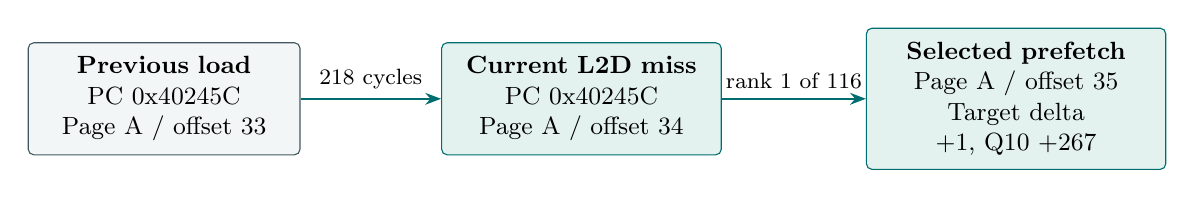
\begin{tikzpicture}[x=1cm,y=1cm,font=\small]
  \node[store,text width=3.1cm] (old) at (1.72,1.25) {\textbf{Previous load}\\PC 0x40245C\\Page A / offset 33};
  \node[block,text width=3.2cm] (now) at (7.02,1.25) {\textbf{Current L2D miss}\\PC 0x40245C\\Page A / offset 34};
  \node[block,text width=3.45cm] (next) at (12.54,1.25) {\textbf{Selected prefetch}\\Page A / offset 35\\Target delta +1, Q10 +267};
  \draw[wire] (old)--node[above,font=\footnotesize] {218 cycles} (now);
  \draw[wire] (now)--node[above,font=\footnotesize] {rank 1 of 116} (next);
\end{tikzpicture}

\textbf{PC} 是执行 load 的指令地址。\textbf{Physical page} 是数据所在的物理页。\textbf{Page offset} 在这里按 cache line 编号。4 KiB 的页有 64 条 64 B 的线，所以编号是 0 到 63。\textbf{Target delta} 表示目标在来源线前后多少条。这里从 offset 34 选 $+1$，地址就是同一页的 offset 35。

Newest 也给 offset 36 打了分。它的 Q10 是 $-1217$，低于 $-950$ 门槛。offset 35 的 $+267$ 过了门槛和缓存检查。V1 的候选规则排除当前页，所以在这次触发上，它的打分器根本看不到 offset 35。

\subhead{这个请求真的来得及吗？}
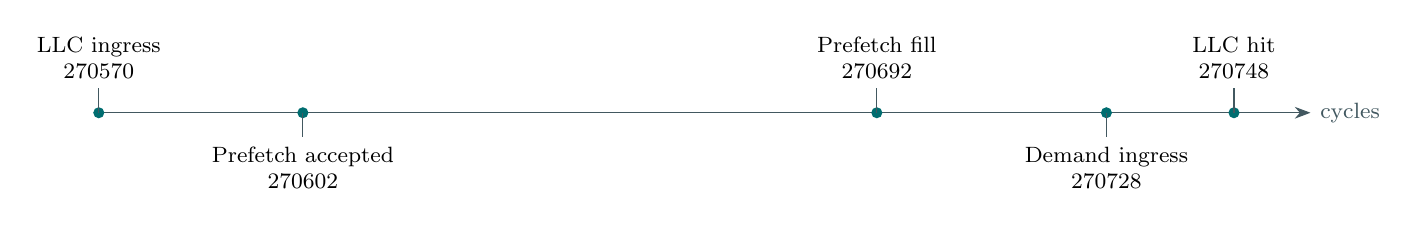
\begin{tikzpicture}[x=.081cm,y=1cm,font=\footnotesize]
  \draw[muted,-{Stealth[length=2mm]}] (0,0)--(190,0) node[right] {cycles};
  \foreach \time/\label/\cycle/\side in {
    0/{LLC ingress}/270570/1,
    32/{Prefetch accepted}/270602/-1,
    122/{Prefetch fill}/270692/1,
    158/{Demand ingress}/270728/-1,
    178/{LLC hit}/270748/1} {
    \fill[teal] (\time,0) circle (2pt);
    \draw[muted] (\time,0)--(\time,{\side*.31});
    \ifnum\side=1
      \node[align=center,anchor=south] at (\time,.31) {\label\\\cycle};
    \else
      \node[align=center,anchor=north] at (\time,-.31) {\label\\\cycle};
    \fi
  }
\end{tikzpicture}\par
同一条目标线的 demand 到 LLC 时，预取已经填好 \textbf{36 cycles}。当前 offset 34 的 L2D miss 本身在 LLC 命中。模型在 LLC 查 tag 之前就看到了这个 L2D miss，因此这样的请求也会更新状态。

\callout{先看同发包量的对照。在原来 90M 和 110M 两段，每版每段都发 2,000 个请求。Newest 的 coverage 分别从 0.754\% 到 2.465\%、从 0.666\% 到 2.820\%。两段合计完成时间基本持平。}

\newpage
\sectionline{MODEL DESIGN}
\titleline{LSTM 记什么，打分器选什么？}
每个 core 维持两条并行信息。一条保存最近读过的地址，告诉模型哪些物理页可以发包。另一条是 LSTM 连续更新的状态，让模型可以根据访问顺序改变分数。两版都只有一层 LSTM，权重在两核间共享，状态按核分开。

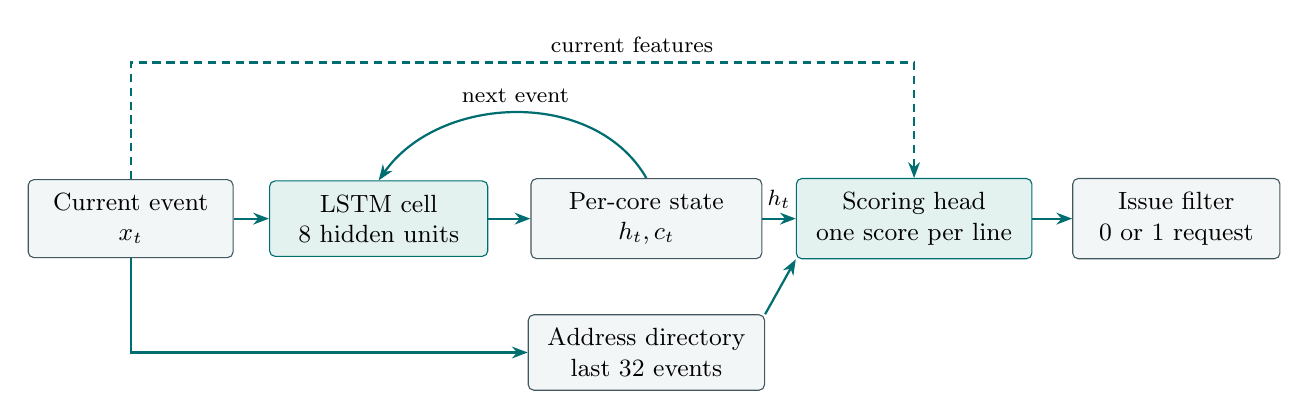
\begin{tikzpicture}[x=1cm,y=1cm,font=\small]
  \node[store,text width=2.25cm] (in) at (1.27,1.73) {Current event\\$x_t$};
  \node[block,text width=2.42cm] (cell) at (4.42,1.73) {LSTM cell\\8 hidden units};
  \node[store,text width=2.58cm] (state) at (7.82,1.73) {Per-core state\\$h_t,c_t$};
  \node[store,text width=2.65cm] (hist) at (7.82,.03) {Address directory\\last 32 events};
  \node[block,text width=2.64cm] (head) at (11.22,1.73) {Scoring head\\one score per line};
  \node[store,text width=2.28cm] (pkt) at (14.55,1.73) {Issue filter\\0 or 1 request};
  \draw[wire] (in)--(cell); \draw[wire] (cell)--(state);
  \draw[wire] (state.north) to[out=120,in=55] node[above,font=\footnotesize] {next event} (cell.north);
  \draw[wire] (state)--node[above,font=\footnotesize] {$h_t$} (head);
  \draw[wire] (hist.north east)--(head.south west);
  \draw[wire] (head)--(pkt);
  \draw[wire] (in.south) |- (hist.west);
  \draw[wire,densely dashed] (in.north) -- ++(0,1.48) -| node[pos=.32,above,font=\footnotesize] {current features} (head.north);
\end{tikzpicture}\par

\subhead{每个输入值有什么用}
{\small
\begin{tabular}{@{}p{2.15cm}>{\raggedright\arraybackslash}p{7.36cm}>{\raggedright\arraybackslash}p{7.37cm}@{}}
\toprule
 & \textbf{V1} & \textbf{Newest}\\
\midrule
Event input & \textbf{7 values}. PC low byte, PC second byte, page offset, same-page delta, page changed, same PC, same line. &
\textbf{9 values}. PC embedding (4), page offset, same-page delta, page changed, same PC, interarrival gap.\\[3pt]
Line or page input & \textbf{6 values per candidate}. Source PC bytes (2), source page offset, target delta, source age in events, source PC matches. &
\textbf{8 values per source page}. Source page offset, source PC embedding (4), current page, source PC matches, source age in cycles.\\[3pt]
Candidate set & Exclude current page. Scan earlier distinct pages in preset four-event age bands. Try
\mbox{$+1,+2,-1,+3,-2,+4,-3,+6,-4,-6$}. Present at most 16 lines to the scorer. &
Use current page and most recent distinct page. Score every legal line in these pages, up to 126. Keep Top 16 after scoring for the issue filter.\\[3pt]
Score & Project $[x_t,h_t]$ to a 4-value query. Project the 6 candidate features to a 4-value key and a bias. The dot product plus bias gives one score. &
Combine $[x_t,h_t]$ with the 8 page features in an 8-unit ReLU head. Each signed target delta has its own weight row and bias.\\
\bottomrule
\end{tabular}\par}

\smallnote{PC 表示哪条指令发来请求。offset 和 page changed 表示地址在哪里、是否换页。delta 表示方向。gap 表示访问来得多密，按 log 档编码，218 cycles 在例子里变成 $7/12$。输入的 same-page delta 比较相邻请求，截到 $\pm8$ 后除以 8。输出的 target delta 用目标线减来源线，范围 $-63$ 到 $+63$。两者来源不同。}

\subhead{四个门如何留下历史}
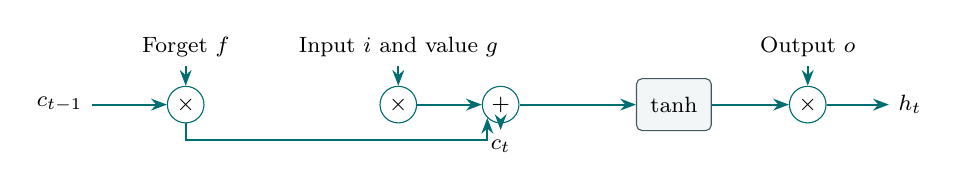
\begin{tikzpicture}[x=1cm,y=.70cm,font=\footnotesize]
  \node (cprev) at (.75,0) {$c_{t-1}$};
  \node[op] (forget) at (2.35,0) {$\times$};
  \node[op] (write) at (5.05,0) {$\times$};
  \node[op] (sum) at (6.35,0) {$+$};
  \node[store] (tanh) at (8.55,0) {$\tanh$};
  \node[op] (read) at (10.25,0) {$\times$};
  \node (h) at (11.55,0) {$h_t$};
  \node (f) at (2.35,1.05) {Forget $f$};
  \node (ig) at (5.05,1.05) {Input $i$ and value $g$};
  \node (o) at (10.25,1.05) {Output $o$};
  \node (c) at (6.35,-.75) {$c_t$};
  \draw[wire] (cprev)--(forget); \draw[wire] (f)--(forget);
  \draw[wire] (ig)--(write); \draw[wire] (write)--(sum);
  \draw[wire] (forget.south) -- ++(0,-.30) -| (sum.south west);
  \draw[wire] (sum)--(c); \draw[wire] (sum)--(tanh);
  \draw[wire] (tanh)--(read); \draw[wire] (o)--(read); \draw[wire] (read)--(h);
\end{tikzpicture}\par
\[
\underbrace{c_t}_{\text{cell state}}
  =\underbrace{f_t}_{\text{forget}}\odot c_{t-1}
   +\underbrace{i_t}_{\text{input}}\odot\underbrace{g_t}_{\text{new content}},
\qquad
\underbrace{h_t}_{\text{hidden state}}
  =\underbrace{o_t}_{\text{output}}\odot\tanh(c_t).
\]
\smallnote{第一页的实测例子里，第一个 cell value 从 $-4.5979$ 开始。Forget $0.8185$，Input $0.8855$，New content $-0.9701$，Output $0.9674$。代入后得到 $c_t\approx-4.6223$，$h_t\approx-0.9673$。这些值和另外七组一起写回该 core 的状态。}

\newpage
\sectionline{TRAINING LABELS}
\titleline{模型怎么知道哪条线值得学？}
先关掉所有预取跑同一段，得到 NoPF demand log。对当前触发和一个合法候选，沿同一 core 的日志查这条线下一次被 demand 访问的时刻和 LLC 结果。未来时刻只写进训练标签。上线时，打分器只收到这个时刻已经观察到的事件。

\subhead{同一个问题，两种标签}
{\small
\begin{tabular}{@{}p{2.35cm}>{\raggedright\arraybackslash}p{7.32cm}>{\raggedright\arraybackslash}p{7.22cm}@{}}
\toprule
 & \textbf{V1 hard label} & \textbf{Newest soft label}\\
\midrule
Target & 下一次同核访问是 NoPF LLC miss，且 lead 在 300–2,000 cycles，取 1。其余取 0。 &
下一次同核访问是 NoPF LLC miss，且 lead 不超过 4,000 cycles，取 $F_S(\max(0,\mathrm{lead}-32))$。其余取 0。\\[3pt]
Why & 用一个固定时间窗挑可能赶上的请求。阈值附近只差一个 cycle 的两个样本也可被分到 0 和 1。&
先留 32 cycles 给预测。剩下的时间越够，标签越高。$F_S$ 是实测 NoPF 服务周期的累计比例。\\
\bottomrule
\end{tabular}\par}

\subhead{回到 Page A、offset 35}
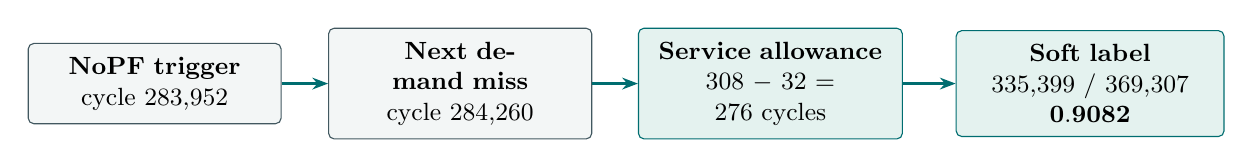
\begin{tikzpicture}[x=1cm,y=1cm,font=\small]
  \node[store,text width=2.86cm] (a) at (1.60,.8) {\textbf{NoPF trigger}\\cycle 283,952};
  \node[store,text width=2.99cm] (b) at (5.48,.8) {\textbf{Next demand miss}\\cycle 284,260};
  \node[block,text width=3.00cm] (c) at (9.42,.8) {\textbf{Service allowance}\\308 $-$ 32 = 276 cycles};
  \node[block,text width=3.05cm] (d) at (13.48,.8) {\textbf{Soft label}\\335,399 / 369,307\\$\mathbf{0.9082}$};
  \draw[wire] (a)--(b); \draw[wire] (b)--(c); \draw[wire] (c)--(d);
\end{tikzpicture}\par
这里是同一动态访问在\textbf{另一遍 NoPF replay}里的周期。offset 35 的标签是 0.9082。同一触发的 offset 36 在 NoPF 里没有后续访问，标签是 0。第一页发包用的 $+267$ 是模型输出的 Q10 score。

\subhead{训练用什么数据}
{\small
\begin{tabular}{@{}p{4.15cm}rr@{}}
\toprule
 & \textbf{V1} & \textbf{Newest}\\
\midrule
Training regions & 10M / 30M / 50M & 10M / 30M / 50M\\
NoPF events & 438,087 & 436,680\\
Valid event--line pairs & 6,995,808 & 54,214,872\\
Nonzero labels & 122,525 & 282,378\\
Selection regions & 70M & 70M / 130M\\
Trained / kept epoch & 4 / 4 & 12 / 8\\
Training block / batch & 256 events / 16 blocks & 128 events / 32 blocks\\
\bottomrule
\end{tabular}\par}
两版都用 PyTorch 的 weighted BCE 和 AdamW，learning rate 0.003，seed 605。正样本少，训练提高正标签的权重。V1 用 Colab CPU，Newest 用本地 PyTorch。训练区间相同，Newest 的 NoPF 事件由本地重新采集。一个 full batch 都有 4,096 个监督事件位置。Newest 多跑几个 epoch，让开发集可以选权重，最终选 epoch 8；训练轮数不改变部署成本。

\smallnote{Newest 的 369,307 个 NoPF service samples 全部来自 10M/30M/50M。p50/p90/p95 是 210/263/340 cycles。两个模型的 checkpoint 在开发段选择，测试段只用于评估。}

\newpage
\sectionline{PARAMETERS AND REPLAY}
\titleline{哪些数字是测出来的，哪些是设计设置？}
{\small
\begin{tabular}{@{}>{\raggedright\arraybackslash}p{3.40cm}>{\raggedright\arraybackslash}p{13.52cm}@{}}
\toprule
\textbf{Setting} & \textbf{Reason and measured cost}\\
\midrule
8 hidden units & 保留 V1 的小状态。每核 $h,c$ 合计 16 个 FP32 值（64 B）。维度扩大时，recurrent matrix 会变大。本次比较固定宽度。\\[2pt]
8-event unroll & V1 在 70M 的 2K/4K offline decisions 下，8、16、32 的去重目标数为 94/130、94/128、94/128。保留 8，训练每 8 条切断梯度。线上 $h,c$ 仍连续传。\\[2pt]
32 directory / 32 burn-in / 128 start & 32-entry directory 找已见地址，按每条 16 B 共 512 B/core。32-event burn-in 给训练块恢复前缀状态。先观察 128 条 ROI 事件，再开始给地址评分。它们各自限制地址存储、训练初始化和发包起点。\\[2pt]
2 pages / 127 target deltas & 当前页补上 V1 漏掉的同页线，再留一个最近不同页的机会。每页 64 条线，位移表有 $2\times64-1=127$ 项。来源线已经访问，从两页扣掉至少两条，最多 126 条可评分。Top 16 把交给后续 filter 的列表控制在原来的大小。\\[2pt]
64 entries $\times$ 4 PC values & 用低 PC bits 折叠成表项，让 PC 作为指令身份学习。64 项共 1,024 B。示例的 PC 0x40245C 访问 entry 5，读出 $[-0.224,-1.908,-1.353,+0.743]$。多个 PC 可以共用表项，维度是存储选择。\\[2pt]
4,000-cycle lookahead & V1 固定窗曾漏掉 2,000 cycles 之后的机会。扩大观察窗口能找到更远的首次 miss。Newest 的训练对中，有 113,047 个 future-miss pairs 的 lead 在 2,000 之后。时间窗仍给日志保留一个固定尾界。\\[2pt]
Q10 / issue threshold & 把 1 个 logit 单位分成 1,024 格，裁成有符号 16 位整数，便于排名。V1 的 $-1037$ 来自 70M 的离线决策阈值。Newest 的 $-950$ 是 70M/130M 上完成周期最短的测试格点，也在该次搜索的下界。\\[2pt]
Runtime cost & V1 / Newest 存 611 / 2,183 个 FP32 系数（2,444 / 8,732 B）。每次触发最多约 1,084 / 1,816 个 matrix MACs。还需地址目录、候选排序、队列与过滤；时钟和面积是后续硬件问题。\\
\bottomrule
\end{tabular}\par}

\subhead{怎么做同条件比较}
同一个 ChampSim-Pythia binary，双核各跑同一份 605 MCF，地址空间分开。每核 200K warmup、2M ROI instructions，4 GHz，4 MiB shared LLC，单通道 DDR4-2400，关闭私有 cache prefetch。两版都用 32-cycle prediction latency、8-cycle initiation interval、每核 4 个在途槽。V1 首次发表的重放用了 16 cycles，这次两版统一到 32 cycles。两核合计 IPC 用实际退休数除以最后一个 core 的完成周期。

\callout{\textbf{No extra cap} 是一个实验开关。两版都用各自冻结的权重和 score threshold。设置 \texttt{issue-limit=0} 时，两版都不额外限制整段的 accepted 数量。每次触发仍最多发 1 个请求，也仍要通过驻留、重复和队列检查。设为 \texttt{1000} 时，每核整段最多发 1,000 个。Newest 在两种条件下都是同一个模型。}

\smallnote{V1 的原测试段是 90M/110M，Newest 的原测试段是 410M/430M/450M。这里用冻结模型重放两组，区间数字指跳过的 trace records。共享上限可以给出不同的实际发包量，图里标的是实数。}

\newpage
\sectionline{RESULTS \quad 1,000 REQUESTS / CORE}
\titleline{先把发包量控制住}
\smallnote{Same total-count ceiling for both. A pair is equal-volume only when its \textbf{Accepted} counts match. V1 uses amber; Newest uses teal. Each row is one complete two-core replay.}
\metricchart{2.06cm}{\qualityheads}{\CapQuality}
\metricchart{2.13cm}{\cacheheads}{\CapCache}

\subhead{原测试段里发生了什么}
90M 和 110M 两版各发 2,000 个请求。覆盖数分别为 \CapNinetyCovered\ 和 \CapOneTenCovered。及时用到的请求从 874 到 1,739，但有用请求中及时的比例从 94.18\% 到 50.38\%。两段合计 15,559,434 $\to$ 15,558,327 cycles，差约 0.007\%。

410M 的 V1 只发 1,571 个，属于相同上限。430M 和 450M 两版都发到 2,000 个。430M 的 coverage 略降，450M 的 coverage 上升但 IPC 降低。四个发包相等的区间合计，coverage 从 0.578\% 到 1.403\%，Newest 完成时间长 0.126\%。

\newpage
\sectionline{RESULTS \quad NO EXTRA TOTAL-COUNT CAP}
\titleline{再看各自冻结策略会实际发多少}
\smallnote{The model and its threshold are unchanged. Both use the same degree and queue checks. This condition measures full-policy behavior at the realized request volumes.}
\metricchart{2.06cm}{\qualityheads}{\NativeQuality}
\metricchart{2.13cm}{\cacheheads}{\NativeCache}

\subhead{这个测试能说明什么}
90M/110M 合计，发包从 5,607 到 43,014，coverage 从 0.769\% 到 25.938\%，执行时间少 4.58\%。410M/430M/450M 合计，发包从 12,097 到 153,362，coverage 从 1.269\% 到 24.308\%，时间少 6.60\%，DRAM 流量从 19.582 到 24.196 MB。这是两个完整策略在各自实际流量下的表现。

\subhead{数字的分母}
\smallnote{\textbf{Accuracy} = useful first uses / accepted requests. \textbf{Timeliness} = timely first uses / useful first uses. \textbf{Coverage} = covered NoPF misses / all NoPF misses. \textbf{Timely coverage} 只计及时覆盖，分母相同。表内 \textbf{Timely} 为对应到 NoPF miss 的及时数。}
\smallnote{按 core、dynamic instruction 和 load operand 匹配 NoPF，并核对 PC 和 virtual line。晚到合并仍算覆盖。LLC hit/miss 以 demand lookups 为分母。MPKI 是每千条退休指令的 misses。Time 由完成周期除以 4 GHz 得到。DRAM MB 包括 demand、prefetch 和 write traffic。}

\newpage
\sectionline{RESULTS \quad 150 REQUESTS / CORE}
\titleline{把两版都压到更小的相同发包量}
\smallnote{An additional matched-count check. The hardware settings and model thresholds stay fixed. Use the Accepted column to distinguish a common limit from equal realized sends.}
\metricchart{2.06cm}{\qualityheads}{\SmallQuality}
\metricchart{2.13cm}{\cacheheads}{\SmallCache}

\subhead{怎么读这组补测}
\SmallBudgetSummary

\smallnote{完整英文 CSV、每核计数、NoPF 分母、真实输入样本和复现代码在 \texttt{lstm/v5\_results/v1\_comparison/}。32-cycle prediction latency 是仿真设定，tag lookup 和 DRAM 服务由模拟器推进。}
\end{document}
